\documentclass{article}
\usepackage{amssymb}
\usepackage{graphicx}
\usepackage{caption}
\usepackage{subcaption}
\usepackage{listings}
\usepackage{float} %figure inside minipage
\graphicspath{ {./images/} }
\usepackage[export]{adjustbox}
\usepackage{apacite}

\begin{document}

\section{Discontinuity in the PDE case}
\subsection{Introduction}
\label{subsection:pde_intro}
In this chapter, we explore the effects of discontinuities on a PDE (partial differential equation) model. We will use an epidemiological model to which we will add a time-dependent discontinuity and a state-dependent discontinuity and report on how the solvers perform.

As was the case with the IVODE model in the previous chapter, PDE models also thrash when they encounter a discontinuity. (See Figure 888888 888888). We thus like investigate the effects of this thrashing on the accuracy and efficiency of PDE models.

\begin{figure}[H]
\centering
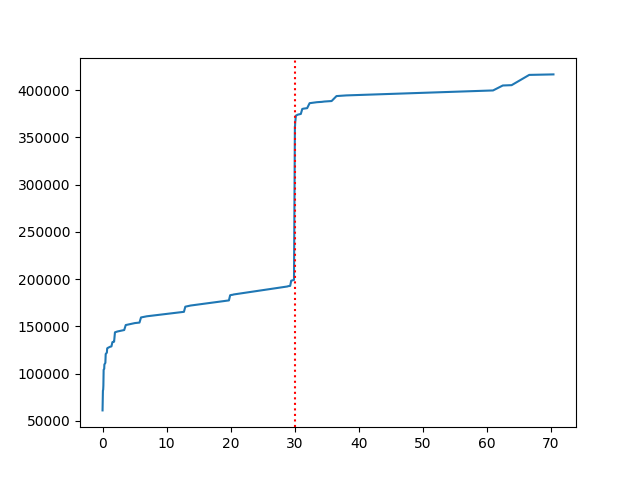
\includegraphics[width=0.7\linewidth]{./figures/PDE_thrashing}
\caption{Thrashing in the PDE context}
\label{fig:thrashing_pde}
\end{figure}

We note that PDE models are often used in epidemiological studies but are very rarely solved with state of the art solvers. In this chapter we will compare [ASK FOR AN OLD solver like EPDCOL or code our own euler method...] against the BACOL family of solvers. (See a description of the software used in Section $\ref{subsection:pde_software}$)

We will show, as was the case in the ODE problem, that thrashing around a discontinuity also happens, that error control can allow us to step through one discontinuity but that the state dependent discontinuity problem can only be solved with event handling. 

\subsubsection{Software used}
\label{subsection:pde_software}
\paragraph{The BACOL family of PDE solvers}
The BACOL family of PDE solvers solve 1D PDEs using B-spline collocation. BACOLI uses DASSL as its DAE solver (which is based on a family of multi-step methods known as the Backward Differentiation Formulas (BDF)) while BACOLRI uses RADAU5 as its DAE solver (which is based on 5th order implicit Runge-Kutta methods). Both have global error control. BACOLIKR is an improvement over BACOLI which uses DASKR instead of DASSL as the DAE solver, allowing it to detect events.

\paragraph{Other Solvers}
[Look for EPDCOL, KARDOS, an euler method and ]


\subsubsection{Problem Definition}
In this paper, the PDE model which we will try to solve is an extension of the SEIR model for epidemiological studies that uses one more spatial variable (x) and not just time. Similar PDE models have been used before 8888 reference to PDE Cholera papers 8888 and either use the spread in location or the age as the additional spatial variable.

The SEIR model was developed by Andrew Fraser 88888 Reference 88888 but some coefficients were changed.

The model is as follows:
\begin{equation}
S(x, t)_t = D_S(x)S(x, t)_{xx} + \mu N - \mu S(x, t) - \frac{\beta}{N}S(x, t) I(x, t)
\end{equation}

\begin{equation}
E(x, t)_t = D_E(x)E(x, t)_{xx} + \frac{\beta}{N}S(x, t)I(x, t) - \alpha E(x, t) - \mu E(x, t)
\end{equation}

\begin{equation}
I(x, t)_t = D_I(x)I(x, t)_{xx} + \alpha E(x, t) - \gamma I(x, t) - \mu I(x, t)
\end{equation}

\begin{equation}
R(x, t)_t = D_R(x)R(x, t)_{xx} + \gamma I(x, t) - \mu R(x, t)
\end{equation} 

The spatial domain is $-5 \leq x \leq 5$ and the temporal domain is $0 \leq t \leq 70$ for the time-dependent discontinuity problem but we will use $0 \leq t \leq 200$ for the space-dependent discontinuity problem as we attempt a long-term forecast.

We use $\frac{0.01}{365}$ as the value of the parameter $\mu$, the birth rate, 0.06 for the value of the recovery rate, $\gamma$, 0.125 as the incubation rate. $\alpha$ and we will vary the transmission rate $\beta$ between 0.9 and 0.005 based on whether measures are implemented or not in the model. The population size, N, is 10.

The model also uses diffusion functions $D_S(x)$, $D_E(x)$, $D_I(x)$ and $D_R(x)$ as follows:

888888888888888888
It is using $sqrt(x^2)$... can I just change it to abs!!! NEED TO CHECK THIS
888888888888888888

\begin{equation}
D_S(x) = D_E(x) = D_R(x) = (maxD_s - minD_s)e^{-10(\sqrt{x^{2}} - 1)^2)} + minD_s
\end{equation} 
\begin{equation}
D_I(x) = D_E(x)/10
\end{equation}

The parameters $maxD_s$ and $minD_s$ are 0.1 and 0.05.

The initial values are functions of the spatial domain as such

\begin{equation}
S(x, 0) = 1 - I(x, 0)
\end{equation}
\begin{equation}
I(x, 0) = 2e^{-10(x+1)^2}
\end{equation}
\begin{equation}
E(x, 0) = R(x, 0) = 0
\end{equation}

This gives us a complete PDE problem definition to which we will add discontinuities as follows. In the time-dependent discontinuity problem, we will integrate the model with $\beta$ at a value of 0.9 from t=0 to t=30, we will then change the value of $\beta$ to 0.005 and integrate until t=70. This change in the parameter introduces a discontinuity.
In the state-dependent discontinuity problem, we integrate with the value of $\beta$ at 0.9 while the integral value of the solution of the E-component is less than 5. When it reaches 5, we integrate with the value of $\beta$ at 0.005 until the integral reaches 1 where we change the value pf $\beta$ back to 0.9. We repeat this process until we reach t=200.

\subsection{Time Dependent Discontinuity}
In this section, we will add a time dependent discontinuity and report on the thrashing experienced by the solvers. We note that this section is in essence an application of what we demonstrated in Section 8888 reference to ODE time dependent 8888 in that time dependent discontinuities are introduced by simply changing a parameter value, as this is essentially changing the model function being integrated and that time-dependent discontinuities have an easy solution by integrating the solution with two calls, one before the discontinuity and one after. This gives the solver two continuous segments to integrate.

In this PDE case, the value of $\beta$ will be 0.9 from t=0 to t=30 and the value of $\beta$ will be changed to 0.005 from t=30 to the end of the integration.

\subsubsection{Naive treatment}
In the naive treatment for this kind of discontinuity is to place the the change in the parameter in the right hand side function as an if-statement. The pseudocode for this approach is as follows:

\begin{minipage}{\linewidth}
\begin{lstlisting}[language=Python]
function model_with_if(t, x, u, ux, uxx)
    // ...
    beta = 0.9
    if t >= 30:
        beta = 0.005
    // ...

\end{lstlisting}
\end{minipage}

This change in the parameter $\beta$ at t=30 introduces a discontinuity as the model function is different. As shown in Section 8888 Refer to section on discontinuity 8888, as the assumptions of continuity of the function and its derivatives no longer hold, the Taylor Series proof of its convergence is no longer valid. However as we have shown in Section 8888 Refer to naive ODE time problem 8888, error-control solver can reduce the step-size extensively to cross one discontinuity.

Here is the result using BACOLI and BACOLRI at a tolerance of $10^{-6}$ for both the absolute and relative tolerances. To allow for comparisons, we use a cross-section at x=0 to show how the model evolves over time.

\begin{figure}[H]
\centering
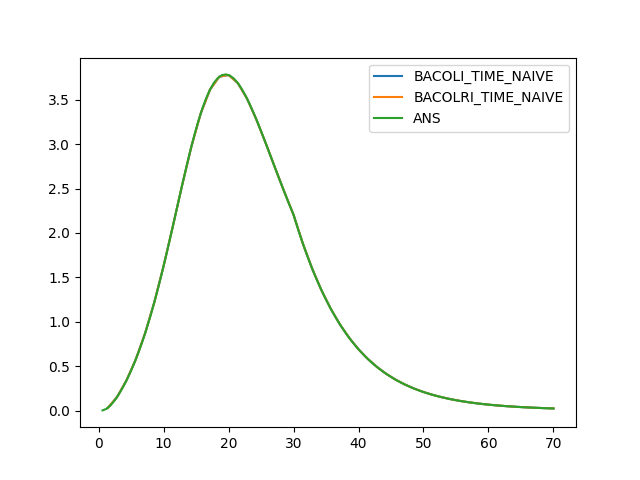
\includegraphics[width=0.7\linewidth]{./figures/pde_time_disc_naive}
\caption{Naive treatment of time discontinuity (at tolerance of $10^{-6}$)}
\label{fig:pde_time_disc_naive}
\end{figure}

From Figure 888 Refer to above figure 888, all the solvers from the BACOL family are able to cross one discontinuity as expected. 
88888 Look to add other solvers - especially non-error control solvers like the ones used in practice 88888


VI VI VI VI VI VI VI VI
BACOLRI nfev DEPENDS ON THE ntout....
VI VI VI VI VI VI VI VI


\subsubsection{Discontinuity handling}
Though the error-controlled solvers were able to get accurate solutions, we now solve the same problem using discontinuity handling. Modern solvers like the BACOL family allows users to set flags to allow it to do a cold start. Thus we integrate the problem with one call from t=0 to t-30 with the model function using 0.9 as the $\beta$ parameter. We then set up a cold start and integrate from t=30 to the end of the time interval with another call to the solver. The pseudo-code is as follows

\begin{minipage}{\linewidth}
\begin{lstlisting}[language=Python]
function model_before(t, x, u, ux, uxx):
    // ...
    beta = 0.9
    // ...
    
function model_after(t, x, u, ux, uxx):
    // ...
    beta = 0.005
    // ...
 
tspan_before = [0, 30]
pde_solver(solution, model_before, tspan_before)

solution.cold_start_flag = True

tspan_after = [30, 70]
pde_solver(solution, model_after, tspan_after)

\end{lstlisting}
\end{minipage}

\begin{figure}[H]
\centering
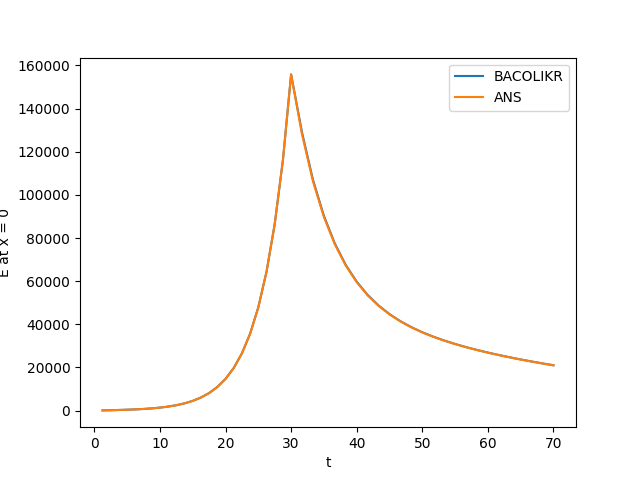
\includegraphics[width=0.7\linewidth]{./figures/pde_time_disc_disc_hand}
\caption{Discontinuity handling for time discontinuity problem (at tolerance of $10^{-6}$)}
\label{fig:pde_time_disc_disc_hand}
\end{figure}

As expected, Figure 888 Refer to above figure 888, the solvers were able to all accurately solve the problem. However, Table $\ref{tab:pde_time_nfev}$ shows how the discontinuity handling allows us to use significantly lower numbers of function evaluations.

\begin{table}[h]
\caption {PDE time discontinuity model} 
\label{tab:pde_time_nfev}
\begin{center}
\begin{tabular}{ c c c } 
method  & no disc. handling & with disc. handling \\ 
BACOLI  & 236715     &   162675     \\
BACOLRI & 238480     &   205540    \\
\end{tabular}
\end{center}
\end{table} 

Table $\ref{tab:pde_time_nfev}$ shows how the use of discontinuity handling in the PDE case also drastically reduces the number of function evaluations. We can see that the number of function evaluations is about half in both cases with the addition of the discontinuity handling. Also, we note that both solvers create B-spline interpolants and thus increasing or reducing the time-grid for plotting does not affect the efficiency. 

\subsubsection{Time problem tolerance study}
In this section, we do a tolerance study on the time dependent problem. We look at how coarse we can reduce the tolerance to still have accurate solution to see if the discontinuity handling allows us to use coarser tolerance as it did in the IVODE case.

\paragraph{BACOLI}

\begin{figure}[H]
\centering
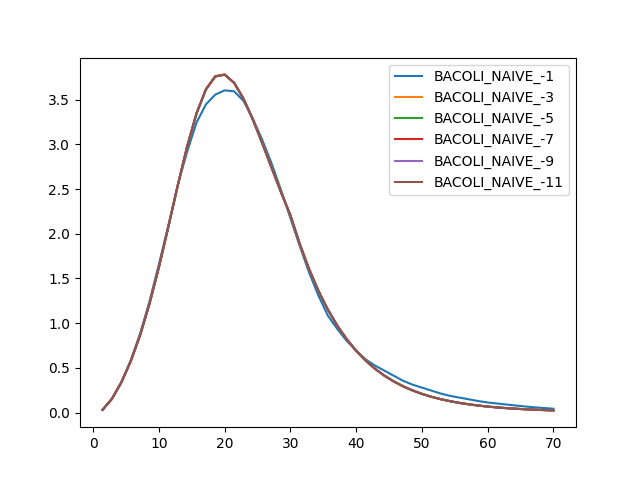
\includegraphics[width=0.7\linewidth]{./figures/pde_time_disc_bacoli_naive_tol}
\caption{Time dependent discontinuity tolerance study with BACOLI using naive treatment}
\label{fig:pde_time_disc_bacoli_naive_tol}
\end{figure}

\begin{figure}[H]
\centering
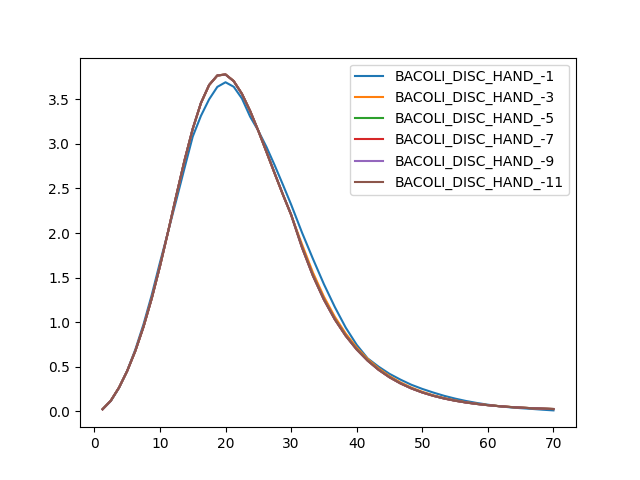
\includegraphics[width=0.7\linewidth]{./figures/pde_time_disc_bacoli_disc_hand_tol}
\caption{Time dependent discontinuity tolerance study with BACOLI using discontinuity handling}
\label{fig:pde_time_disc_bacoli_disc_hand_tol}
\end{figure}

\begin{table}[h]
\caption {BACOLI time discontinuity model tolerance study} 
\label{tab:BACOLI_time_tolerance}
\begin{center}
\begin{tabular}{ c c c } 
tolerance  & BACOLI naive & BACOLI with disc handling\\ 
1e-1       & 44730        &   46410     \\
1e-3       & 58950        &   51750    \\
1e-5       & 129305       &   101025    \\
1e-7       & 371210       &   294770    \\
1e-9       & 1100095      &   773040    \\
1e-11      & 3120140      &   2337900    \\
\end{tabular}
\end{center}
\end{table}

\paragraph{BACOLRI}

\begin{figure}[H]
\centering
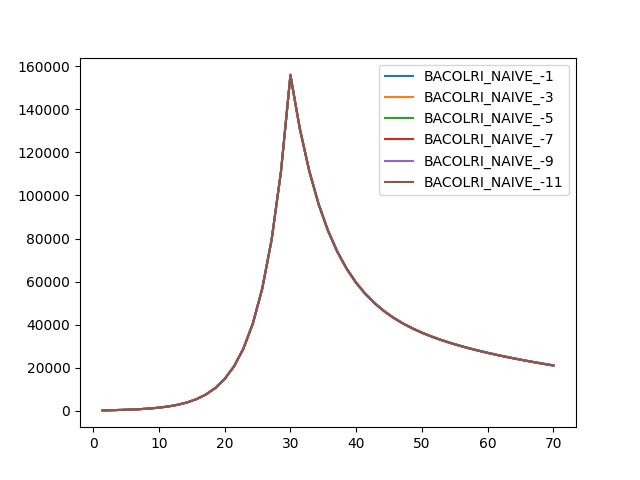
\includegraphics[width=0.7\linewidth]{./figures/pde_time_disc_bacolri_naive_tol}
\caption{Time dependent discontinuity tolerance study with BACOLRI using naive treatment}
\label{fig:pde_time_disc_bacolri_naive_tol}
\end{figure}

\begin{figure}[H]
\centering
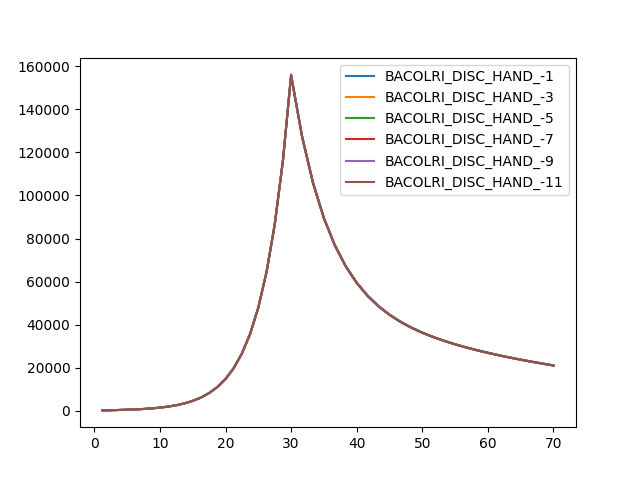
\includegraphics[width=0.7\linewidth]{./figures/pde_time_disc_bacolri_disc_hand_tol}
\caption{Time dependent discontinuity tolerance study with BACOLRI using discontinuity handling}
\label{fig:pde_time_disc_bacolri_disc_hand_tol}
\end{figure}

\begin{table}[h]
\caption {BACOLRI time discontinuity model tolerance study} 
\label{tab:BACOLRI_time_tolerance}
\begin{center}
\begin{tabular}{ c c c } 
tolerance  & BACOLRI naive & BACOLRI with disc handling\\ 
1e-1       & 82595        &   81020     \\
1e-3       & 88220        &   85475    \\
1e-5       & 166150       &   156540    \\
1e-7       & 353875       &   331095    \\
1e-9       & 818395       &   771685    \\
1e-11      & 2189820      &   2165290    \\
\end{tabular}
\end{center}
\end{table}

\subsection{State Dependent Discontinuity}
In this section, we discuss a state-dependent discontinuity problem in that we compare the current value of the state or one of its component against a predetermined threshold and if that threshold is crossed, we change the model equation. Unlike, in the IVODE case, we need to account for the spatial domain when finding the state value to compare against a threshold. Some of the ways to do so are listed below:
\begin{itemize}
\item Pick a spatial value, say x = 0, and sample the state value at this spatial point at every time interval. If the state value meets a certain threshold, we apply a different model, else we use the same model

\item Find some statistic measure (min, max, mean, median) across the spatial domain and use that value for the comparison with the threshold.

\item Integrate over the spatial domain and use that integral value for the comparison against the threshold.
\end{itemize}

In this report we will use the third method in that we will integrate over the spatial domain. If the value of the integral crosses a maximum threshold (integral value of 5) while measures are not implemented, the value of the parameter $\beta$ is changed from 0.9 to 0.005 and if measures are implemented and we cross a certain minimum threshold (integral value of 1), the value of the parameter $\beta$ is changed back to 0.9. This is repeated several time for the time period t=0 to t=200.  

We note that the discontinuity is introduced by the change in the parameter $\beta$ and which method to obtain the state value at a certain time does not matter, so the conclusions of this paper equally applies to the other methods of finding the state value at a given time.
 
\subsubsection{Naive Treatment}
For the naive treatment of this problem, a user will use a boolean for whether measures are implemented or not, as a global variable. This global variable is toggled based on the integral value over the spatial domain at a given time.  

To perform the integration the naive user will have to do a manual time stepping. The user will divide the time into equal intervals and once they reach the end of the time interval, they will make an interpolant over the spatial domain at that time and integrate it. 

If measures are not implemented and the integral is greater than 5, the maximum threshold, they will switch the global variable indicating that measures are implemented. When there are no measures implemented, the user will integrate at the end of a step and look for an integral value less than 1, the minimum threshold. When such an integral value is less than 1, the user will switch the global variable indicating that measures are no longer implemented. When measures are implemented, the value of the parameter $\beta$ is 0.005 while it is 0.9 when measures are not implemented. 

The pseudocode for this approach is as shown:

\begin{minipage}{\linewidth}
\begin{lstlisting}[language=Python]
measures_implemented = False

function model(t, x, u, ux, uxx):
    // ...
    if (measures_implemented):
    		beta = 0.005
    	else:
    		beta = 0.9
    // ...

tstart = 0
tstop = 200
num_times = 400
time_step_size = (tstop - tstart) / num_times
		
t_current = tstart
t_next = t_current + time_step_size

while t_current < tstop:
	tspan = [t_current, t_next]
	pde_solver(solution, model, tspan)
	
	integral_value = integrate(interpolate(solution))
	
	if (measures_implemented):
		if (integral_value >= 6):
			measures_implemented = True
	else:
		if (integral_value <= 1):
			measures_implemented = False
	
	t_current = t_next
	t_next = t_next + time_step_size
\end{lstlisting}
\end{minipage}

The pseudo-code shows a clear problem with the naive solution. The user has an additional variable, the number of time steps, to set. The number of time steps needs to be big enough that we know when the threshold are met but need to be small enough that the integration can occur without issue. 

The solution on solving this problem with a naive solution is as shown in Figures 8888 8888 and 8888 8888 where the number of time steps is 200 and 400 respectively. 

\begin{figure}[H]
\centering
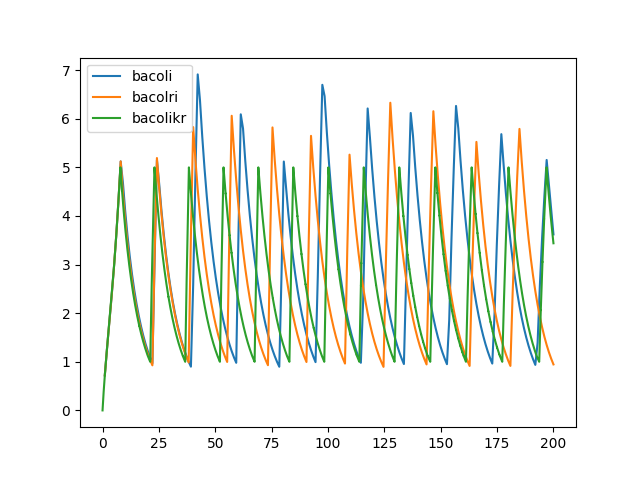
\includegraphics[width=0.7\linewidth]{./figures/pde_state_disc_naive_200}
\caption{State dependent discontinuity naive treatment with a tolerance of $10^{-6}$ and 200 time steps}
\label{fig:pde_state_disc_naive_200}
\end{figure}

\begin{figure}[H]
\centering
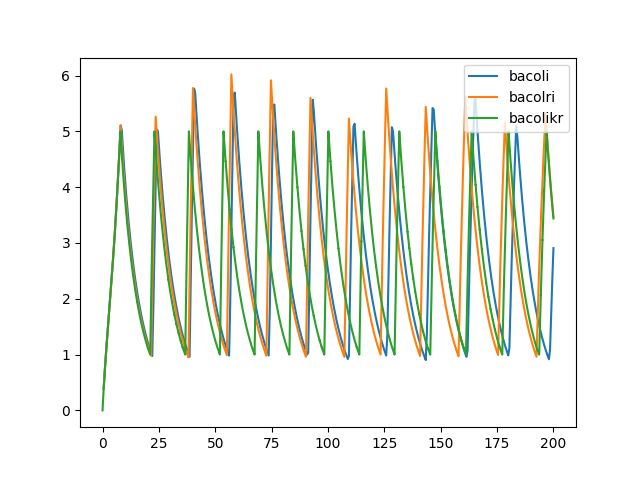
\includegraphics[width=0.7\linewidth]{./figures/pde_state_disc_naive_400}
\caption{State dependent discontinuity naive treatment with a tolerance of $10^{-6}$ and 400 time steps}
\label{fig:pde_state_disc_naive_400}
\end{figure}

\subsubsection{Why the naive method cannot give an accurate solution}
The naive method cannot solve the problem accurately because of the problem of choosing a correct number of time steps to perform the spatial integration. We note that most of the time, the method will find the correct integral value much after it crosses the threshold and not exactly when it does so. This means that we take up to one additional time step with the previous $\beta$ value and not the correct one.

One idea to solve this problem would be to use an exceedingly large number of time steps (1000 in our case) such that we take the smallest step possible with the old value. This, however, reduces the efficiency, making us do more time steps than necessary. (See efficiency comparisons in Table 8888 Refer to table in next section 8888). The best solution is to use event detection.

\begin{figure}[H]
\centering
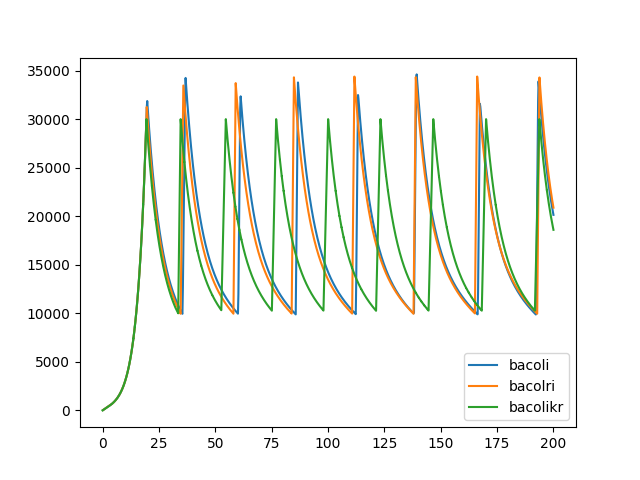
\includegraphics[width=0.7\linewidth]{./figures/pde_state_disc_naive_1000}
\caption{State dependent discontinuity naive treatment with a tolerance of $10^{-6}$ and 1000 time steps}
\label{fig:pde_state_disc_naive_1000}
\end{figure}
 
From the above, we can see that a high enough number of time steps allow us to get better and better solution...

\subsubsection{Event Detection solution}
As was the case in the IVODE case, event detection is also present in some PDE solvers. Event detection works in the same way: the user provides a root function to the PDE solver, after each time step the solver calls the root function with the solution at the current time step and stores its value. If the value returned by the root function changes sign, the PDE solvers employs a root-finding routine to find where the root function is zero exactly. The solver then returns, setting a flags indicating that it has found a root with the values at the root.
 
For the BACOL family of PDE solver, BACOLIKR is an improvement to the BACOLI solver which has root finding capabilities. Instead of using DASSL as its DAE solver, it uses DASKR which can detect roots as its solves a DAE system. We use BACOLIKR to demonstrate that using a PDE SOLVER with root-finding capabilities allows us to not define a time grid and thus allows us to integrate with the best accuracy-efficiency trade-off.  

We define two pairs of root and model functions. One pair is to be used when integrating when there are no measures in place. The model function will have the variable $\beta$ at a value of 0.9 and the root function will do the integration of the spatial domain at the current time step and will return if it is closed to the maximum threshold. 5. The second pair will have the model function with $\beta$ at a value of 0.005 and the root function looking for a root at 1. The pseudo-code for this approach is as follows:

\begin{minipage}{\linewidth}
\begin{lstlisting}[language=Python]
function model_no_measures(t, x, u, ux, uxx):
	// ...
	beta = 0.9
	// ...
	
function root_max_value(t, solution):
	// ...
	integral_value = integrate(interpolate(solution))
	return integral_value - 5
	
function model_with_measures(t, x, u, ux, uxx):
	// ...
	beta = 0.005
	// ...
	
function root_min_value(t, solution):
	// ...
	integral_value = integrate(interpolate(solution))
	return integral_value - 1


tstart = 0
tstop = 200
		
t_current = tstart
measures_implemented = false

while t_current < tstop:
	tspan = [t_current, t_stop]
	if (measures_implemented):
		pde_solver(solution, model_with_measures, tspan, root_min_value)
	else:
		pde_solver(solution, model_no_measures, tspan, root_max_value)
		
	if (solution.root_flag == True):
		# root detected, if a max root, add measures else remove measures
		solution.cold_start_flag = True
		if (measures_implemented):
			measures_implemented = False
		else:
			measures_implemented = True
		
	t_current = solution.t

\end{lstlisting}
\end{minipage}


\begin{figure}[H]
\centering
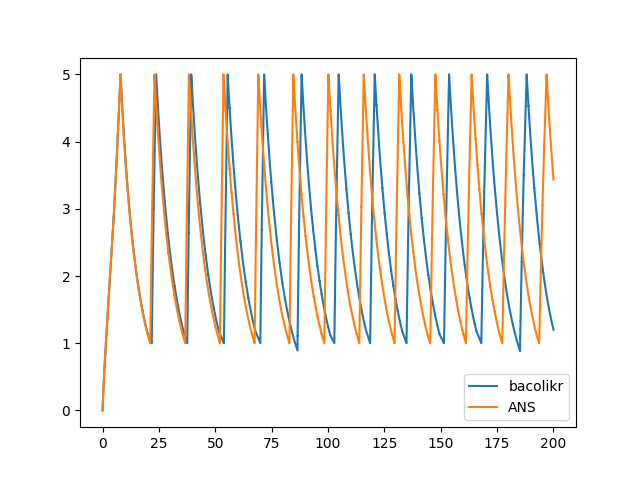
\includegraphics[width=0.7\linewidth]{./figures/pde_state_disc_event_tol_6}
\caption{State dependent discontinuity using event detection with a tolerance of $10^{-6}$}
\label{fig:pde_state_disc_event_tol_6}
\end{figure}

As we can see, we get a solution that oscillates correctly. However the two solutions are not correctly aligned, especially at lower time period. We will see that the tolerance need to be high enough

\begin{figure}[H]
\centering
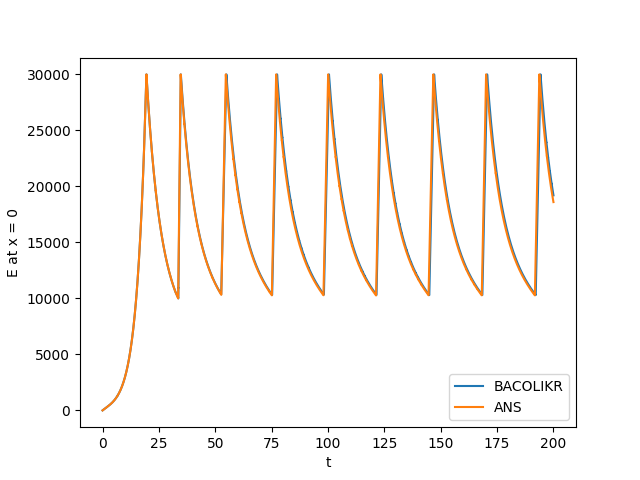
\includegraphics[width=0.7\linewidth]{./figures/pde_state_disc_event_tol_9}
\caption{State dependent discontinuity using event detection with a tolerance of $10^{-9}$}
\label{fig:pde_state_disc_event_tol_9}
\end{figure}

From Figure 8888 8888, we can see that with event detection, it is only a matter of tolerance to see whether the answer is correct...

\begin{table}[h]
\caption {PDE state discontinuity model} 
\label{tab:pde_state_nfev}
\begin{center}
\begin{tabular}{ c c } 
method                  & nfev \\ 
BACOLI 200 steps        & 784230    \\
BACOLI 400 steps        & 813555    \\
BACOLI 1000 steps       & 874605    \\
BACOLRI 200 steps       & 612100    \\
BACOLRI 400 steps       & 1075835    \\
BACOLRI 1000 steps      & 3354275    \\
BACOLIKR tol $10^{-6}$  & 1067420    \\
BACOLIKR tol $10^{-9}$  & 4996210    \\
\end{tabular}
\end{center}
\end{table} 

\subsubsection{State problem tolerance study}
We also perform a tolerance study at 400 and at 1000 to show how the solutions compare for all the solvers. We try to look for why even BACOLIKR does not solve the problem and look to see if there is anything we can do

\paragraph{BACOLI}
\begin{figure}[H]
\centering
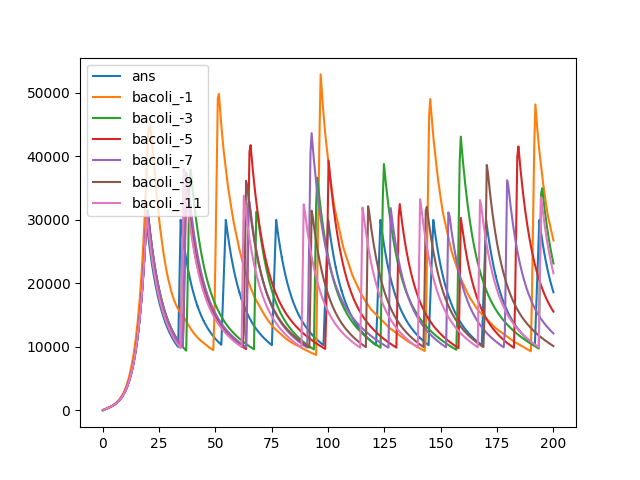
\includegraphics[width=0.7\linewidth]{./figures/pde_state_disc_tol_bacoli_400}
\caption{State dependent discontinuity naive treatment tolerance study with BACOLI with 400 time steps}
\label{fig:pde_state_disc_tol_bacoli_400}
\end{figure}

\begin{figure}[H]
\centering
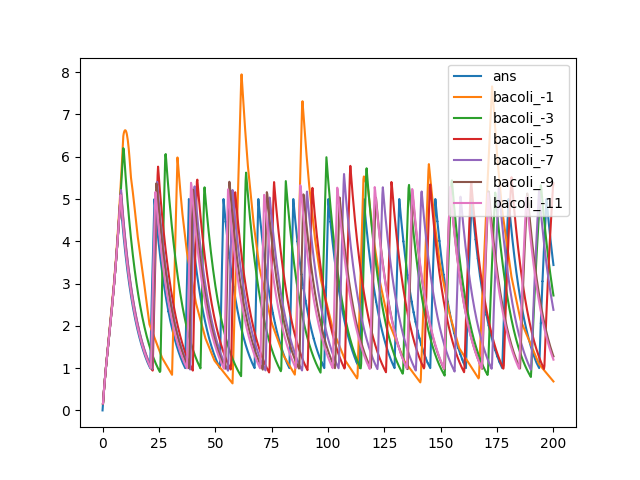
\includegraphics[width=0.7\linewidth]{./figures/pde_state_disc_tol_bacoli_1000}
\caption{State dependent discontinuity naive treatment tolerance study with BACOLI with 1000 time steps}
\label{fig:pde_state_disc_tol_bacoli_1000}
\end{figure}

\paragraph{BACOLRI}
\begin{figure}[H]
\centering
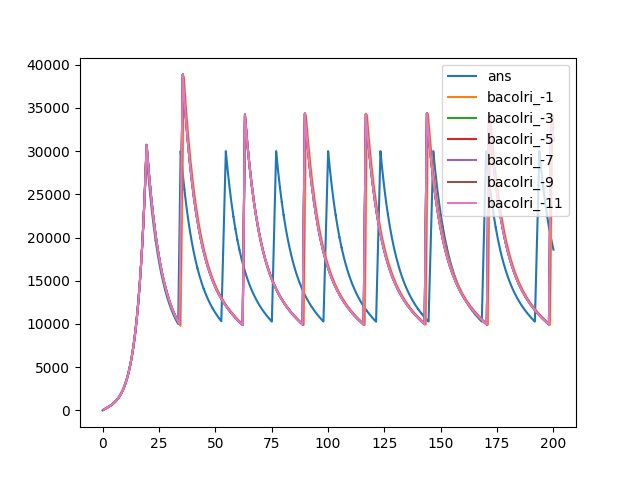
\includegraphics[width=0.7\linewidth]{./figures/pde_state_disc_tol_bacolri_400}
\caption{State dependent discontinuity naive treatment tolerance study with BACOLRI with 400 time steps}
\label{fig:pde_state_disc_tol_bacolri_400}
\end{figure}

\begin{figure}[H]
\centering
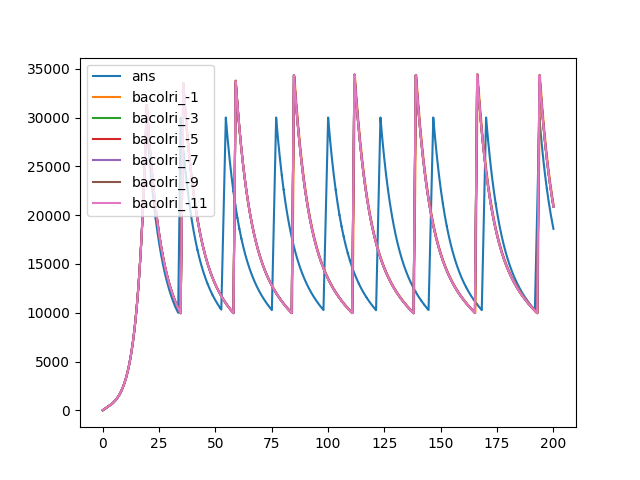
\includegraphics[width=0.7\linewidth]{./figures/pde_state_disc_tol_bacolri_1000}
\caption{State dependent discontinuity naive treatment tolerance study with BACOLRI with 1000 time steps}
\label{fig:pde_state_disc_tol_bacolri_1000}
\end{figure}

\paragraph{BACOLIKR}
\begin{figure}[H]
\centering
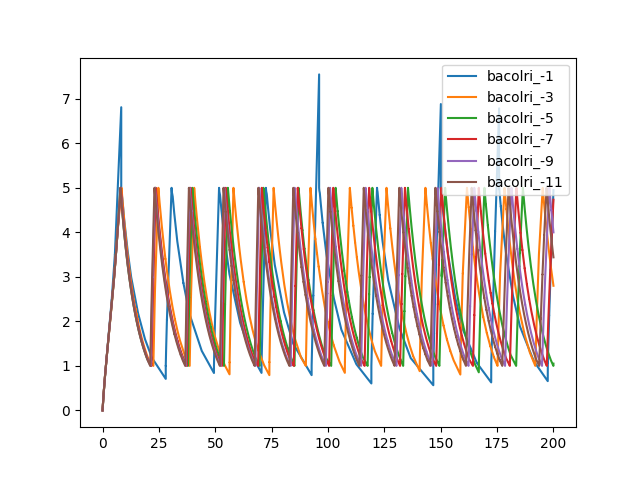
\includegraphics[width=0.7\linewidth]{./figures/pde_state_disc_tol_event}
\caption{State dependent discontinuity using event detection tolerance study}
\label{fig:pde_state_disc_tol_event}
\end{figure}

\paragraph{number of function evaluations}

\begin{table}[h]
\caption {BACOLRI time discontinuity model} 
\label{tab:BACOLRI_time_tolerance}
\begin{center}
\begin{tabular}{ c c c c c c } 
tolerance  & BACOLIKR  & BACOLI 400   & BACOLI 1000 & BACOLRI 400 & BACOLRI 1000\\ 
1e-3       & 333700    &   330750     & 340650      & 638120      & 1582760   \\
1e-5       & 801530    &   524595     & 599425      & 1018550     & 2520970  \\
1e-7       & 2091040   &   1331390    & 1358950     & 1509400     & 4266070 \\
1e-9       & 4996210   &   3967825    & 4176470     & 3148635     & 7223550 \\
1e-11      & 13031060  &   10687490   & 10565330    & 7467960     & 14833180  \\
\end{tabular}
\end{center}
\end{table}


VI VI VI VI VI VI VI VI VI VI

BACOLRI CAN GET THE CORRECT VALUE if the time grid is sharp enough => see plot of 400 vs 800

It seems that with a dense enough grid, the non-event detection solvers could eventually solve the problem...
More strangely, BACOLRI seems to always give the same incorrect solution at the different tolerances showing that the time step IS THE ONLY LIMITING FACTOR FOR IT...
This is in contrast with BACOLI....
However if we increase the tolerance of DASSL for BACOLI, we get the same results.... 


VI VI VI VI VI VI VI VI VI VI

\subsection{Discussions}

\end{document}
